%\VignetteEngine{knitr::knitr}
%\VignetteIndexEntry{Flexible Logo plots of symbols and alphanumeric strings using Logolas}
%\VignettePackage{CountClust}

% To compile this document
% library('knitr'); rm(list=ls()); knit('Logolas/vignettes/logolas.Rnw')
% library('knitr'); rm(list=ls()); knit2pdf('Logolas/vignettes/logolas.Rnw'); openPDF('logolas.pdf')
% !Rnw weave = knitr

\documentclass[12pt]{article}\usepackage[]{graphicx}\usepackage[usenames,dvipsnames]{color}
%% maxwidth is the original width if it is less than linewidth
%% otherwise use linewidth (to make sure the graphics do not exceed the margin)
\makeatletter
\def\maxwidth{ %
  \ifdim\Gin@nat@width>\linewidth
    \linewidth
  \else
    \Gin@nat@width
  \fi
}
\makeatother

\definecolor{fgcolor}{rgb}{0.345, 0.345, 0.345}
\newcommand{\hlnum}[1]{\textcolor[rgb]{0.686,0.059,0.569}{#1}}%
\newcommand{\hlstr}[1]{\textcolor[rgb]{0.192,0.494,0.8}{#1}}%
\newcommand{\hlcom}[1]{\textcolor[rgb]{0.678,0.584,0.686}{\textit{#1}}}%
\newcommand{\hlopt}[1]{\textcolor[rgb]{0,0,0}{#1}}%
\newcommand{\hlstd}[1]{\textcolor[rgb]{0.345,0.345,0.345}{#1}}%
\newcommand{\hlkwa}[1]{\textcolor[rgb]{0.161,0.373,0.58}{\textbf{#1}}}%
\newcommand{\hlkwb}[1]{\textcolor[rgb]{0.69,0.353,0.396}{#1}}%
\newcommand{\hlkwc}[1]{\textcolor[rgb]{0.333,0.667,0.333}{#1}}%
\newcommand{\hlkwd}[1]{\textcolor[rgb]{0.737,0.353,0.396}{\textbf{#1}}}%

\usepackage{framed}
\makeatletter
\newenvironment{kframe}{%
 \def\at@end@of@kframe{}%
 \ifinner\ifhmode%
  \def\at@end@of@kframe{\end{minipage}}%
  \begin{minipage}{\columnwidth}%
 \fi\fi%
 \def\FrameCommand##1{\hskip\@totalleftmargin \hskip-\fboxsep
 \colorbox{shadecolor}{##1}\hskip-\fboxsep
     % There is no \\@totalrightmargin, so:
     \hskip-\linewidth \hskip-\@totalleftmargin \hskip\columnwidth}%
 \MakeFramed {\advance\hsize-\width
   \@totalleftmargin\z@ \linewidth\hsize
   \@setminipage}}%
 {\par\unskip\endMakeFramed%
 \at@end@of@kframe}
\makeatother

\definecolor{shadecolor}{rgb}{.97, .97, .97}
\definecolor{messagecolor}{rgb}{0, 0, 0}
\definecolor{warningcolor}{rgb}{1, 0, 1}
\definecolor{errorcolor}{rgb}{1, 0, 0}
\newenvironment{knitrout}{}{} % an empty environment to be redefined in TeX

\usepackage{alltt}

\newcommand{\Logolas}{\textit{Logolas}}
\usepackage{dsfont}
\usepackage{cite}



\RequirePackage{/Library/Frameworks/R.framework/Versions/3.3/Resources/library/BiocStyle/resources/tex/Bioconductor}

\AtBeginDocument{\bibliographystyle{/Library/Frameworks/R.framework/Versions/3.3/Resources/library/BiocStyle/resources/tex/unsrturl}}



\author{Kushal K Dey \\[1em]
\small{\textit{Stephens Lab}, The University of Chicago} \mbox{ }\\
\small{\texttt{$^*$Correspondending Email: kkdey@uchicago.edu}}}


\bioctitle[ Flexible Logo plots of symbols and alphanumeric strings using \Logolas{}]{Flexible Logo plots of alphanumeric strings and symbols using \Logolas{}}
\IfFileExists{upquote.sty}{\usepackage{upquote}}{}
\begin{document}

\maketitle

\begin{abstract}
  \vspace{1em}
Logo plots are popular in genomic studies for sequence alignment and motif detection. However, logos have been pretty restrictive in its scope because of limited library of symbols it uses and the lack of flexibility in extending it to other applications. In this package, we provide an easy and more flexible interface for the user to plot logos and more importantly, we extend the library of logos from A, C, T, G (as in seqLogo) and English alphabets (RWebLogo) to include numbers and alpha-numeric strings with provision for punctuations and arrows. It also provides the user with a simple interface to create her own logo and add to her personal library.
In this vignette, we discuss a number of applications beyond sequence alignment where such flexible logo plots can be used.
\end{abstract}

\vspace{1em}
\textbf{\Logolas{} version:} 0.1.0 \footnote{This document used the vignette from \Bioconductor{} package \Biocpkg{CountClust, DESeq2} as \CRANpkg{knitr} template}
\end{abstract}




\newpage

\tableofcontents

\section{Introduction}

Logo plots are a popular tool in bioinformatics and regulatory genomics studies for representing sequence alignment patterns and also sequence and protein motif detection. One of the first logo plotting tools is \Biocpkg{seqLogo} by Oliver Bembom \cite{Bembom2016}, specifically targeted at DNA sequence alignment. However, it has a library of only 4 symbols - A, C, G and T- corresponding to the 4 nucleotides. The package \CRANpkg{RWebLogo} is an extension of WebLogo python package that plots custom sequence logos by extending it to all alphabets. Another package \Biocpkg{motifStack} works with both DNA/RNA sequence motif and amino acid sequence motif and customizes font size and colors.

\Logolas{} adds more flexibility by customizing logos and the graphical design of the logo plots. Also it extends the library of symbols beyond English alphabets to numbers, symbols (arrows, punctuations) and to alphanumeric strings. It allows the user to choose a range of information criteria to determine logo sizes and more importantly, a simple user interface to create new logos and add them to the library of logos already present and to strings. We show several applications in genomics, ecology and document mining, where such logo plots can be applied.

\section{\Logolas{} Installation}

\Logolas{} requires the following CRAN-R package : \CRANpkg{grid}, \CRANpkg{gridExtra}, \CRANpkg{RColorBrewer}, \CRANpkg{devtools}.

\begin{knitrout}
\definecolor{shadecolor}{rgb}{0.969, 0.969, 0.969}\color{fgcolor}\begin{kframe}
\begin{alltt}
\hlkwd{source}\hlstd{(}\hlstr{"http://bioconductor.org/biocLite.R"}\hlstd{)}
\hlkwd{biocLite}\hlstd{(}\hlstr{"Logolas"}\hlstd{)}
\end{alltt}
\end{kframe}
\end{knitrout}

For the developmental version on Github, one can use

\begin{knitrout}
\definecolor{shadecolor}{rgb}{0.969, 0.969, 0.969}\color{fgcolor}\begin{kframe}
\begin{alltt}
\hlkwd{install_github}\hlstd{(}\hlstr{'kkdey/Logolas'}\hlstd{)}
\end{alltt}
\end{kframe}
\end{knitrout}

Then load the package with:

\begin{knitrout}
\definecolor{shadecolor}{rgb}{0.969, 0.969, 0.969}\color{fgcolor}\begin{kframe}
\begin{alltt}
\hlkwd{library}\hlstd{(Logolas)}
\end{alltt}
\end{kframe}
\end{knitrout}

\section{Application}

We start with the most basic application of logo plots - for alignment of DNA sequence, comprising of logos A, C, T and G, corresponding to the four nucleotide. This is the typical application of \Biocpkg{seqLogo}. We start with a demo example and apply \Biocpkg{seqLogo} to it.

\begin{figure}[h]
\begin{center}
\begin{knitrout}
\definecolor{shadecolor}{rgb}{0.969, 0.969, 0.969}\color{fgcolor}\begin{kframe}
\begin{alltt}
\hlkwd{library}\hlstd{(seqLogo)}
\hlstd{mFile} \hlkwb{<-} \hlkwd{system.file}\hlstd{(}\hlstr{"Exfiles/pwm1"}\hlstd{,} \hlkwc{package}\hlstd{=}\hlstr{"seqLogo"}\hlstd{)}
\hlstd{m} \hlkwb{<-} \hlkwd{read.table}\hlstd{(mFile)}
\hlstd{p} \hlkwb{<-} \hlkwd{makePWM}\hlstd{(m)}
\hlkwd{seqLogo}\hlstd{(p)}
\end{alltt}
\end{kframe}
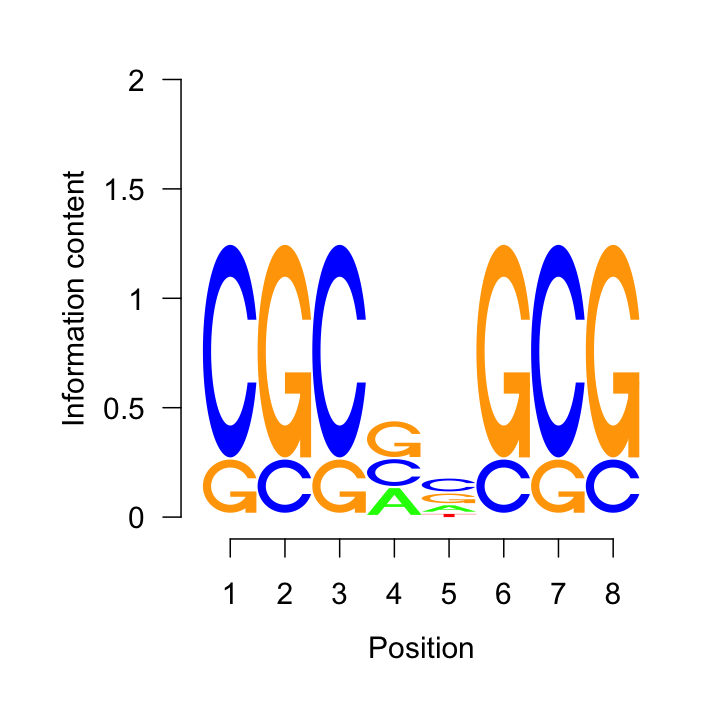
\includegraphics[width=5in,height=5in]{figure/seqlogo_use-1} 

\end{knitrout}
\end{center}
\end{figure}


The user first needs to make a position weight matrix from the matrix using the \begin{verb} makePWM() \end{verb} function. Then it uses the \begin{verb} seqLogo() \end{verb} function on the output to plot the logo plots.

\newpage

Now we apply \Logolas{} to build similar plot. We start with the same matrix as in \Biocpkg{seqLogo}, and assign row names and column names that will be used in the plot as symbols and block labels respectively.

\begin{figure}[h]
\begin{center}
\begin{knitrout}
\definecolor{shadecolor}{rgb}{0.969, 0.969, 0.969}\color{fgcolor}\begin{kframe}
\begin{alltt}
\hlkwd{rownames}\hlstd{(m)} \hlkwb{<-} \hlkwd{c}\hlstd{(}\hlstr{"A"}\hlstd{,} \hlstr{"C"}\hlstd{,} \hlstr{"G"}\hlstd{,} \hlstr{"T"}\hlstd{)}
\hlkwd{colnames}\hlstd{(m)} \hlkwb{<-} \hlnum{1}\hlopt{:}\hlnum{8}
\hlkwd{logomaker}\hlstd{(m,}
          \hlkwc{cols}\hlstd{= RColorBrewer}\hlopt{::}\hlkwd{brewer.pal}\hlstd{(}\hlkwd{dim}\hlstd{(m)[}\hlnum{1}\hlstd{],}\hlkwc{name} \hlstd{=}\hlstr{"Spectral"}\hlstd{),}
          \hlkwc{frame_width} \hlstd{=} \hlnum{1}\hlstd{,}
          \hlkwc{ic.scale} \hlstd{=} \hlnum{TRUE}\hlstd{,}
          \hlkwc{yscale_change}\hlstd{=}\hlnum{FALSE}\hlstd{,}
          \hlkwc{xlab}\hlstd{=}\hlstr{"position"}\hlstd{,}
          \hlkwc{col_line_split} \hlstd{=} \hlstr{"grey80"}\hlstd{)}
\end{alltt}
\end{kframe}
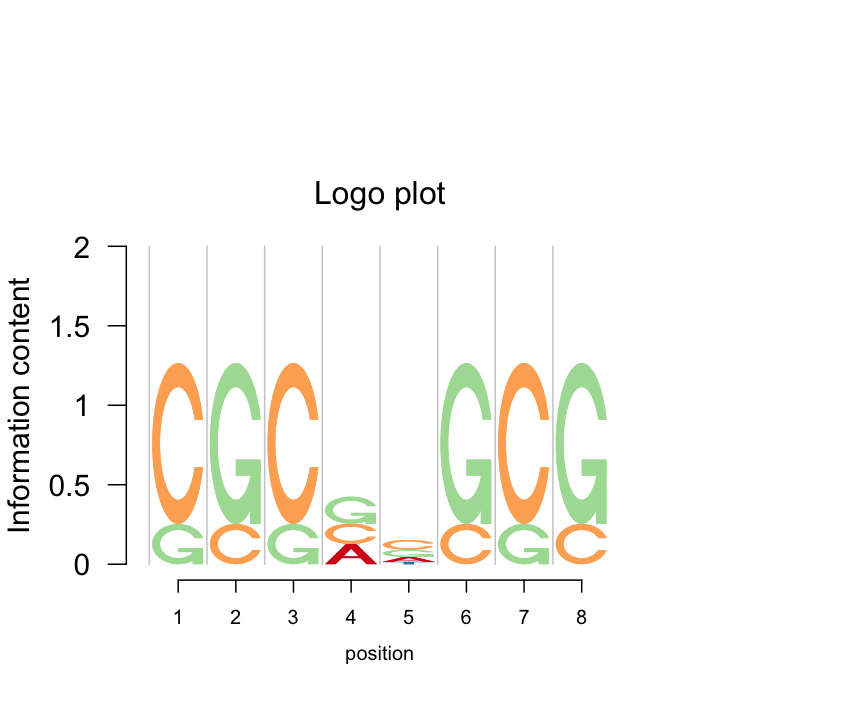
\includegraphics[width=6in,height=5in]{figure/logolas_use-1} 

\end{knitrout}
\end{center}
\end{figure}

\newpage

As default, if \begin{verb} ic.scale = TRUE \end{verb}, the heights of the bars at each position are determined by the Shannon entropy. The size of logo in each stack is proportional to the relative abundance of that logo in that stack. To change to other orders of Renyi entropy, one can tune the input parameter \begin{verb} alpha \end{verb}.

A higher value of  \begin{verb} alpha \end{verb} makes the logos more prominent, besides maintaining relative structure.

Also, the Y-axis can be adjusted by taking \begin{verb} yscale_change=TRUE \end{verb}

\begin{figure}[h]
\begin{center}
\begin{knitrout}
\definecolor{shadecolor}{rgb}{0.969, 0.969, 0.969}\color{fgcolor}\begin{kframe}
\begin{alltt}
\hlkwd{rownames}\hlstd{(m)} \hlkwb{<-} \hlkwd{c}\hlstd{(}\hlstr{"A"}\hlstd{,} \hlstr{"C"}\hlstd{,} \hlstr{"G"}\hlstd{,} \hlstr{"T"}\hlstd{)}
\hlkwd{colnames}\hlstd{(m)} \hlkwb{<-} \hlnum{1}\hlopt{:}\hlnum{8}
\hlkwd{logomaker}\hlstd{(m,}
          \hlkwc{cols}\hlstd{= RColorBrewer}\hlopt{::}\hlkwd{brewer.pal}\hlstd{(}\hlkwd{dim}\hlstd{(m)[}\hlnum{1}\hlstd{],}\hlkwc{name} \hlstd{=}\hlstr{"Spectral"}\hlstd{),}
          \hlkwc{frame_width} \hlstd{=} \hlnum{1}\hlstd{,}
          \hlkwc{ic.scale} \hlstd{=} \hlnum{TRUE}\hlstd{,}
          \hlkwc{alpha} \hlstd{=} \hlnum{2}\hlstd{,}
          \hlkwc{yscale_change}\hlstd{=}\hlnum{FALSE}\hlstd{,}
          \hlkwc{xlab}\hlstd{=}\hlstr{"position"}\hlstd{,}
          \hlkwc{col_line_split} \hlstd{=} \hlstr{"grey80"}\hlstd{)}
\end{alltt}
\end{kframe}
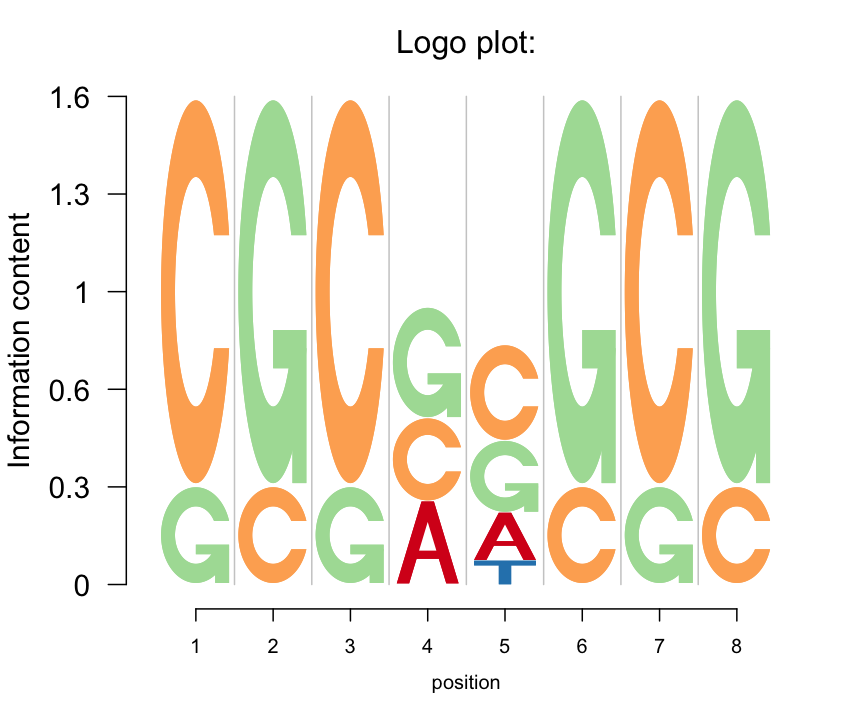
\includegraphics[width=6in,height=5in]{figure/logolas_use_2-1} 

\end{knitrout}
\end{center}
\end{figure}


\newpage

One can also use normalized heights of the stacks of logos for each column by choosing \begin{verb} ic.scale = FALSE \end{verb}.

\begin{figure}[h]
\begin{center}
\begin{knitrout}
\definecolor{shadecolor}{rgb}{0.969, 0.969, 0.969}\color{fgcolor}\begin{kframe}
\begin{alltt}
\hlkwd{rownames}\hlstd{(m)} \hlkwb{<-} \hlkwd{c}\hlstd{(}\hlstr{"A"}\hlstd{,} \hlstr{"C"}\hlstd{,} \hlstr{"G"}\hlstd{,} \hlstr{"T"}\hlstd{)}
\hlkwd{colnames}\hlstd{(m)} \hlkwb{<-} \hlnum{1}\hlopt{:}\hlnum{8}
\hlkwd{logomaker}\hlstd{(m,}
          \hlkwc{cols}\hlstd{= RColorBrewer}\hlopt{::}\hlkwd{brewer.pal}\hlstd{(}\hlkwd{dim}\hlstd{(m)[}\hlnum{1}\hlstd{],}\hlkwc{name} \hlstd{=}\hlstr{"Spectral"}\hlstd{),}
          \hlkwc{frame_width} \hlstd{=} \hlnum{1}\hlstd{,}
          \hlkwc{ic.scale} \hlstd{=} \hlnum{FALSE}\hlstd{,}
          \hlkwc{alpha} \hlstd{=} \hlnum{2}\hlstd{,}
          \hlkwc{xlab}\hlstd{=}\hlstr{"position"}\hlstd{,}
          \hlkwc{col_line_split} \hlstd{=} \hlstr{"grey80"}\hlstd{)}
\end{alltt}
\end{kframe}
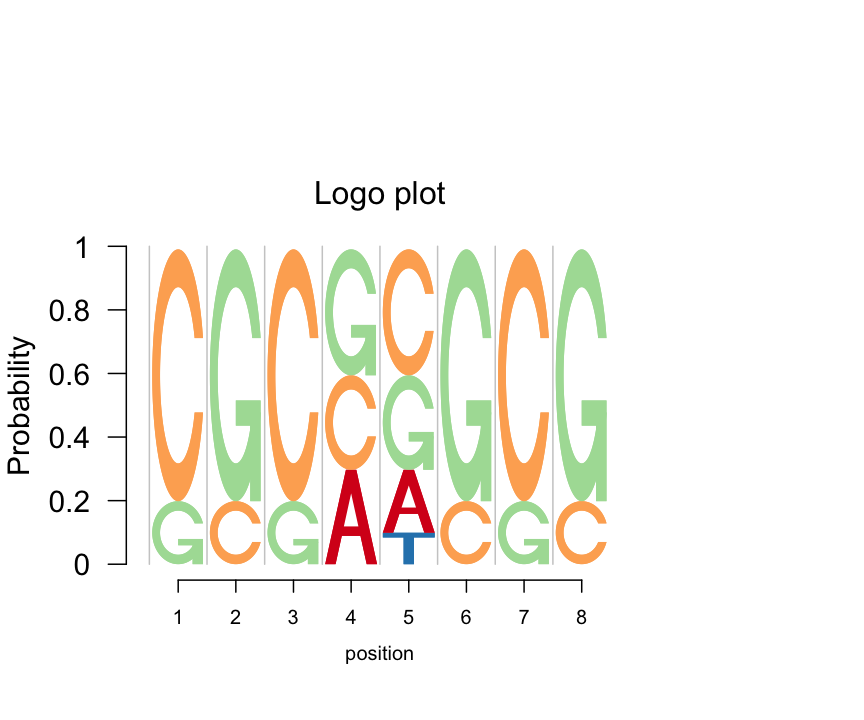
\includegraphics[width=6in,height=5in]{figure/logolas_use_3-1} 

\end{knitrout}
\end{center}
\end{figure}







\end{document}
